\documentclass[aspectratio=169]{beamer}

% Dependency setup
\usepackage{tikz}
\usetikzlibrary{decorations.markings}
%

% Beamer styling setup
\usetheme{AnnArbor}
\usecolortheme{beaver}
\setbeamercolor{titlelike}{parent=structure,bg=gray!15}
\setbeamertemplate{navigation symbols}{}
%

% Beamer notes setup
\usepackage{pgfpages}
% \setbeameroption{show notes on second screen=right}
%

% Spacing setup
\setlength{\parindent}{0pt} % No paragraph indenting
\setlength{\parskip}{5pt} % Set spacing between paragraphs
\frenchspacing
\newcommand{\mkspace}{\vspace{19pt}}
\newcommand{\rmspace}{\vspace{-19pt}}
\newcommand{\emptyline}{\vspace{\baselineskip}}
%

\begin{document}
\title{Paraméteres bonyolultság}
\author{Kovács Milán, Nemkin Viktória}
\date{2021. március 16.}

\AtBeginSection[]
{
    \begin{frame}
        \frametitle{Menetrend}
        \tableofcontents[currentsection]
    \end{frame}
}

\frame{\titlepage}

\frame{\frametitle{Menetrend}\tableofcontents}

\section{Motiváció}
\begin{frame}
\frametitle{Klasszikus bonyolultságelmélet}

Algoritmus: hány lépést tesz az input méretének függvényében?

\begin{itemize}
\item Nem biztos, hogy az egyforma méretű bemenetek egyformán nehezek...
\item Nem biztos, hogy egy teljesen általános megoldásra van szükségünk...
\end{itemize}

\end{frame}


\begin{frame}[t]
\frametitle{Példa: Prímtényezős felbontás}

Feladat: számok prímtényezős felbontását megadni.

\mkspace
\begin{columns}
\begin{column}{0.487\textwidth}
$4503599627370496 = 2^{52}$
\end{column}
\begin{column}{0.487\textwidth}
$1125897758834689 = 524287 \cdot 2147483647$
\end{column}
\end{columns}
\mkspace

\begin{itemize}
\item Input mérete: 16 számjegy.
\item Kézzel melyiket fogjuk tudni hamarabb megadni?
\item Számítógép: sokkal több számjegyre hasonlóan (pl. csak 10-nél kisebb prímek vannak benne $\leftrightarrow$ RSA kódolás).
\end{itemize}

\note{Ugyanolyan sok számjegyből állnak a számok, tehát ugyanolyan hosszú az input méretünk, mégis az elsőt
nagyon gyorsan meg lehet találni, a másodikat sokkal lassabban.}

\end{frame}


\begin{frame}
\begin{footnotesize}
\frametitle{Példa: Sűrű / ritka gráfok}
\note{Everything you want}

\begin{columns}
\begin{column}{0.5\textwidth}
Sűrű gráf:
\begin{center}
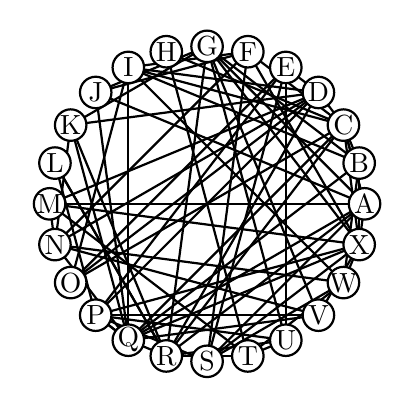
\begin{tikzpicture}[scale=2]
\coordinate (A) at (2.00000,1.00000);
\coordinate (B) at (1.96593,1.25882);
\coordinate (C) at (1.86603,1.50000);
\coordinate (D) at (1.70711,1.70711);
\coordinate (E) at (1.50000,1.86603);
\coordinate (F) at (1.25882,1.96593);
\coordinate (G) at (1.00000,2.00000);
\coordinate (H) at (0.74118,1.96593);
\coordinate (I) at (0.50000,1.86603);
\coordinate (J) at (0.29289,1.70711);
\coordinate (K) at (0.13397,1.50000);
\coordinate (L) at (0.03407,1.25882);
\coordinate (M) at (0.00000,1.00000);
\coordinate (N) at (0.03407,0.74118);
\coordinate (O) at (0.13397,0.50000);
\coordinate (P) at (0.29289,0.29289);
\coordinate (Q) at (0.50000,0.13397);
\coordinate (R) at (0.74118,0.03407);
\coordinate (S) at (1.00000,0.00000);
\coordinate (T) at (1.25882,0.03407);
\coordinate (U) at (1.50000,0.13397);
\coordinate (V) at (1.70711,0.29289);
\coordinate (W) at (1.86603,0.50000);
\coordinate (X) at (1.96593,0.74118);
\draw[thick] (B) -- (Q);
\draw[thick] (G) -- (V);
\draw[thick] (R) -- (U);
\draw[thick] (M) -- (X);
\draw[thick] (P) -- (P);
\draw[thick] (G) -- (U);
\draw[thick] (N) -- (M);
\draw[thick] (B) -- (I);
\draw[thick] (F) -- (N);
\draw[thick] (Q) -- (N);
\draw[thick] (A) -- (S);
\draw[thick] (N) -- (V);
\draw[thick] (X) -- (B);
\draw[thick] (B) -- (X);
\draw[thick] (J) -- (A);
\draw[thick] (T) -- (R);
\draw[thick] (F) -- (X);
\draw[thick] (N) -- (W);
\draw[thick] (V) -- (Q);
\draw[thick] (Q) -- (C);
\draw[thick] (R) -- (G);
\draw[thick] (Q) -- (R);
\draw[thick] (J) -- (F);
\draw[thick] (M) -- (D);
\draw[thick] (C) -- (H);
\draw[thick] (G) -- (A);
\draw[thick] (T) -- (U);
\draw[thick] (P) -- (Q);
\draw[thick] (H) -- (T);
\draw[thick] (P) -- (U);
\draw[thick] (C) -- (D);
\draw[thick] (S) -- (X);
\draw[thick] (S) -- (F);
\draw[thick] (X) -- (A);
\draw[thick] (I) -- (W);
\draw[thick] (I) -- (O);
\draw[thick] (I) -- (Q);
\draw[thick] (A) -- (C);
\draw[thick] (D) -- (O);
\draw[thick] (C) -- (A);
\draw[thick] (G) -- (J);
\draw[thick] (V) -- (X);
\draw[thick] (I) -- (D);
\draw[thick] (R) -- (D);
\draw[thick] (R) -- (C);
\draw[thick] (O) -- (E);
\draw[thick] (L) -- (P);
\draw[thick] (L) -- (R);
\draw[thick] (Q) -- (X);
\draw[thick] (W) -- (T);
\draw[thick] (E) -- (P);
\draw[thick] (K) -- (R);
\draw[thick] (S) -- (P);
\draw[thick] (U) -- (E);
\draw[thick] (V) -- (P);
\draw[thick] (R) -- (R);
\draw[thick] (E) -- (D);
\draw[thick] (B) -- (G);
\draw[thick] (M) -- (T);
\draw[thick] (N) -- (D);
\draw[thick] (D) -- (K);
\draw[thick] (X) -- (C);
\draw[thick] (C) -- (I);
\draw[thick] (N) -- (K);
\draw[thick] (A) -- (Q);
\draw[thick] (G) -- (X);
\draw[thick] (E) -- (S);
\draw[thick] (M) -- (A);
\draw[thick] (P) -- (X);
\draw[thick] (W) -- (S);
\draw[thick] (F) -- (I);
\draw[thick] (M) -- (M);
\draw[thick] (R) -- (A);
\draw[thick] (Q) -- (K);
\draw[thick] (R) -- (L);
\draw[thick] (Q) -- (P);
\draw[thick] (J) -- (Q);
\draw[thick] (P) -- (D);
\draw[thick] (G) -- (K);
\draw[thick] (W) -- (X);
\draw[thick] (C) -- (B);
\draw[thick] (W) -- (W);
\draw[thick] (F) -- (C);
\draw[thick] (O) -- (C);
\draw[thick] (H) -- (H);
\draw[thick] (W) -- (B);
\draw[thick, fill=white] (A) circle (0.1) node {A};
\draw[thick, fill=white] (B) circle (0.1) node {B};
\draw[thick, fill=white] (C) circle (0.1) node {C};
\draw[thick, fill=white] (D) circle (0.1) node {D};
\draw[thick, fill=white] (E) circle (0.1) node {E};
\draw[thick, fill=white] (F) circle (0.1) node {F};
\draw[thick, fill=white] (G) circle (0.1) node {G};
\draw[thick, fill=white] (H) circle (0.1) node {H};
\draw[thick, fill=white] (I) circle (0.1) node {I};
\draw[thick, fill=white] (J) circle (0.1) node {J};
\draw[thick, fill=white] (K) circle (0.1) node {K};
\draw[thick, fill=white] (L) circle (0.1) node {L};
\draw[thick, fill=white] (M) circle (0.1) node {M};
\draw[thick, fill=white] (N) circle (0.1) node {N};
\draw[thick, fill=white] (O) circle (0.1) node {O};
\draw[thick, fill=white] (P) circle (0.1) node {P};
\draw[thick, fill=white] (Q) circle (0.1) node {Q};
\draw[thick, fill=white] (R) circle (0.1) node {R};
\draw[thick, fill=white] (S) circle (0.1) node {S};
\draw[thick, fill=white] (T) circle (0.1) node {T};
\draw[thick, fill=white] (U) circle (0.1) node {U};
\draw[thick, fill=white] (V) circle (0.1) node {V};
\draw[thick, fill=white] (W) circle (0.1) node {W};
\draw[thick, fill=white] (X) circle (0.1) node {X};
\end{tikzpicture}
\end{center}

\end{column}

\begin{column}{0.5\textwidth}
Ritka gráf:
\begin{center}
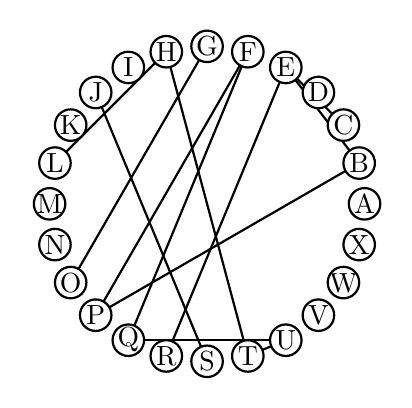
\begin{tikzpicture}[scale=2]
\coordinate (A) at (2.00000,1.00000);
\coordinate (B) at (1.96593,1.25882);
\coordinate (C) at (1.86603,1.50000);
\coordinate (D) at (1.70711,1.70711);
\coordinate (E) at (1.50000,1.86603);
\coordinate (F) at (1.25882,1.96593);
\coordinate (G) at (1.00000,2.00000);
\coordinate (H) at (0.74118,1.96593);
\coordinate (I) at (0.50000,1.86603);
\coordinate (J) at (0.29289,1.70711);
\coordinate (K) at (0.13397,1.50000);
\coordinate (L) at (0.03407,1.25882);
\coordinate (M) at (0.00000,1.00000);
\coordinate (N) at (0.03407,0.74118);
\coordinate (O) at (0.13397,0.50000);
\coordinate (P) at (0.29289,0.29289);
\coordinate (Q) at (0.50000,0.13397);
\coordinate (R) at (0.74118,0.03407);
\coordinate (S) at (1.00000,0.00000);
\coordinate (T) at (1.25882,0.03407);
\coordinate (U) at (1.50000,0.13397);
\coordinate (V) at (1.70711,0.29289);
\coordinate (W) at (1.86603,0.50000);
\coordinate (X) at (1.96593,0.74118);
\draw[thick] (T) -- (H);
\draw[thick] (Q) -- (U);
\draw[thick] (P) -- (F);
\draw[thick] (S) -- (J);
\draw[thick] (C) -- (E);
\draw[thick] (B) -- (P);
\draw[thick] (G) -- (O);
\draw[thick] (Q) -- (F);
\draw[thick] (E) -- (B);
\draw[thick] (H) -- (L);
\draw[thick] (E) -- (R);
\draw[thick] (T) -- (U);
\draw[thick, fill=white] (A) circle (0.1) node {A};
\draw[thick, fill=white] (B) circle (0.1) node {B};
\draw[thick, fill=white] (C) circle (0.1) node {C};
\draw[thick, fill=white] (D) circle (0.1) node {D};
\draw[thick, fill=white] (E) circle (0.1) node {E};
\draw[thick, fill=white] (F) circle (0.1) node {F};
\draw[thick, fill=white] (G) circle (0.1) node {G};
\draw[thick, fill=white] (H) circle (0.1) node {H};
\draw[thick, fill=white] (I) circle (0.1) node {I};
\draw[thick, fill=white] (J) circle (0.1) node {J};
\draw[thick, fill=white] (K) circle (0.1) node {K};
\draw[thick, fill=white] (L) circle (0.1) node {L};
\draw[thick, fill=white] (M) circle (0.1) node {M};
\draw[thick, fill=white] (N) circle (0.1) node {N};
\draw[thick, fill=white] (O) circle (0.1) node {O};
\draw[thick, fill=white] (P) circle (0.1) node {P};
\draw[thick, fill=white] (Q) circle (0.1) node {Q};
\draw[thick, fill=white] (R) circle (0.1) node {R};
\draw[thick, fill=white] (S) circle (0.1) node {S};
\draw[thick, fill=white] (T) circle (0.1) node {T};
\draw[thick, fill=white] (U) circle (0.1) node {U};
\draw[thick, fill=white] (V) circle (0.1) node {V};
\draw[thick, fill=white] (W) circle (0.1) node {W};
\draw[thick, fill=white] (X) circle (0.1) node {X};
\end{tikzpicture}
\end{center}

\end{column}
\end{columns}

Erre a két gráfra nézzünk gráfalgoritmusokat:
\begin{itemize}
\item Legnagyobb független csúcshalmaz.
\item Csúcsszínezés.
\item Stb...
\end{itemize}

Mindkét gráfban ugyanannyi csúcs van, ezért ha szomszédossági mátrixukkal adjuk meg őket, akkor
ugyanakkora lesz az input mérete, azonban a 2. gráfban a fenti kérdésekre elég hamar választ
tudunk adni.
\end{footnotesize}
\end{frame}


\begin{frame}
\frametitle{Valós életbeli problémák}

Üzleti korlátok:

\begin{itemize}
\item Facebook:
\begin{itemize}
\item ismerősök száma $\leq{}$ 500 (fokszám)
\item aktív felhasználók száma $\leq{}$ 3 milliárd (csúcsszám)
\end{itemize}
\item Google:
\begin{itemize}
\item keresett kifejezés hossza $\leq{}$ 100 karakter (illesztett minta hossza)
\item egy oldalon a linkek száma $\leq{}$ 1000 (fokszám)
\end{itemize}
\item Orvosi alkalmazások:
\begin{itemize}
\item DNS hosszúsága
\item protein max mérete
\end{itemize}
\end{itemize}
...stb
\end{frame}




\section{Bar Fight Prevention problem}
\input{02_bar_fight_prevention_problem/01_sztori}
\begin{frame}
\frametitle{Bar Fight Prevention problem}

Input
\begin{itemize}
\item Vendégek listája: n darab vendég
\item Minden vendégpárra: fognak-e verekedni
\item Legfeljebb hány vendéget utasíthatunk el: k (kevesebbet lehet)
\end{itemize}

Output
\begin{itemize}
\item Megoldható-e, hogy a beengedettek között ne legyen verekedés?
\item Kiket kell kitiltani?
\end{itemize}

\end{frame}


\begin{frame}
\frametitle{Példa}

\begin{center}
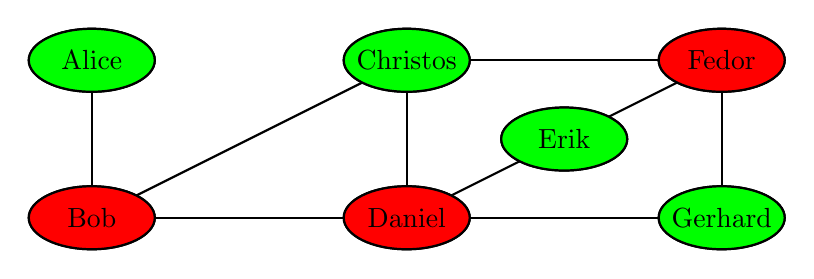
\begin{tikzpicture}[scale=2]
\coordinate (A) at (1,2);
\coordinate (B) at (1,1);
\coordinate (C) at (3,2);
\coordinate (D) at (3,1);
\coordinate (E) at (4,1.5);
\coordinate (F) at (5,2);
\coordinate (G) at (5,1);

\draw[thick] (B) -- (D);
\draw[thick] (D) -- (G);
\draw[thick] (C) -- (F);

\draw[thick] (B) -- (A);
\draw[thick] (D) -- (C);
\draw[thick] (G) -- (F);

\draw[thick] (B) -- (C);
\draw[thick] (D) -- (E);
\draw[thick] (E) -- (F);

\uncover<1>{\draw[thick, fill=white] (A) ellipse (0.4 and 0.2) node {Alice};}
\uncover<2>{\draw[thick, fill=green] (A) ellipse (0.4 and 0.2) node {Alice};}

\uncover<1>{\draw[thick, fill=white] (B) ellipse (0.4 and 0.2) node {Bob};}
\uncover<2>{\draw[thick, fill=red  ] (B) ellipse (0.4 and 0.2) node {Bob};}

\uncover<1>{\draw[thick, fill=white] (C) ellipse (0.4 and 0.2) node {Christos};}
\uncover<2>{\draw[thick, fill=green] (C) ellipse (0.4 and 0.2) node {Christos};}

\uncover<1>{\draw[thick, fill=white] (D) ellipse (0.4 and 0.2) node {Daniel};}
\uncover<2>{\draw[thick, fill=red  ] (D) ellipse (0.4 and 0.2) node {Daniel};}

\uncover<1>{\draw[thick, fill=white] (E) ellipse (0.4 and 0.2) node {Erik};}
\uncover<2>{\draw[thick, fill=green] (E) ellipse (0.4 and 0.2) node {Erik};}

\uncover<1>{\draw[thick, fill=white] (F) ellipse (0.4 and 0.2) node {Fedor};}
\uncover<2>{\draw[thick, fill=red  ] (F) ellipse (0.4 and 0.2) node {Fedor};}

\uncover<1>{\draw[thick, fill=white] (G) ellipse (0.4 and 0.2) node {Gerhard};}
\uncover<2>{\draw[thick, fill=green] (G) ellipse (0.4 and 0.2) node {Gerhard};}

\end{tikzpicture}
\end{center}

\begin{footnotesize}
\begin{itemize}
\item Csúcsok = vendégek, élek = verekedni fognak.
\item Kitilható vendégek száma: k=3.
\end{itemize}
Kérdések:
\begin{itemize}
\item Kit tiltsunk ki, hogy ne legyen verekedés? \\
\uncover<2>{\textcolor{red}{Bob-ot, Daniel-t és Fedor-t.}}
\item Melyik Algoritmuselméletből tanult feladat ez? \\
\uncover<2>{\textcolor{red}{Lefogó csúcshalmaz: $\forall$ él legalább egyik végpontja benne van.}}
\end{itemize}
\end{footnotesize}
\end{frame}


\begin{frame}
\frametitle{Brute force megoldás}
\begin{itemize}
\item Brute force algoritmus.
\item Minden lehetséges részhalmazt megnézzük: ha őket dobnánk ki a többiek verekednének-e?
\item $2^n$, pl n=1000-re már túl nagy.
\end{itemize}
\end{frame}


\begin{frame}
\frametitle{Paraméter választás\uncover<2>{: fokszám}}

\begin{columns}
\begin{column}{0.5\textwidth}
\begin{footnotesize}
\begin{itemize}
\item Csúcsok száma: $n$ (pl. $1000$)
\item
\only<1>{Kizárható vendégek száma: $k$ (pl. $10$)}
\only<2>{\textcolor{red}{Még kizárható vendégek száma: $k'\leq{}k$ (pl. $10$)}}
\uncover<2>{\item\textcolor{red}{Csúcsok fokszáma: $1\leq{}d(v)\leq{}k'$}}
\end{itemize}
\emptyline
Mit tehetünk a következő csúcsokkal?
\begin{itemize}
\item A: $0$ fokszámú csúcs\\
\uncover<2>{\footnotesize{\textcolor{red}{$\rightarrow$ Beengedhető, nem ronthatja el}}}
\item B: $k+1\leq$ fokszámú csúcs\\
\uncover<2>{\footnotesize{\textcolor{red}{$\rightarrow$ Mindenképp ki kell zárni}}}\\
\uncover<2>{\footnotesize{\textcolor{red}{$\rightarrow$ k' = k-1 kizárás maradt}}}
\end{itemize}
\end{footnotesize}
\end{column}

\begin{column}{0.5\textwidth}
\begin{center}
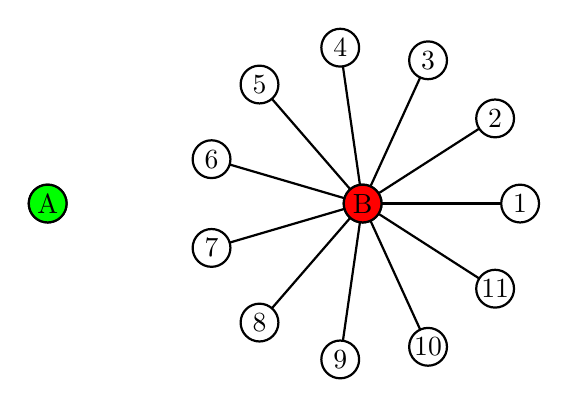
\begin{tikzpicture}[scale=2]
\coordinate (N1)  at (3.00000,1.00000);
\coordinate (N2)  at (2.84125,1.54064);
\coordinate (N3)  at (2.41542,1.90963);
\coordinate (N4)  at (1.85769,1.98982);
\coordinate (N5)  at (1.34514,1.75575);
\coordinate (N6)  at (1.04051,1.28173);
\coordinate (N7)  at (1.04051,0.71827);
\coordinate (N8)  at (1.34514,0.24425);
\coordinate (N9)  at (1.85769,0.01018);
\coordinate (N10) at (2.41542,0.09037);
\coordinate (N11) at (2.84125,0.45936);
\coordinate (A)   at (0.00000,1.00000);
\coordinate (B)   at (2.00000,1.00000);
\draw[thick] (B) -- (N1);
\draw[thick] (B) -- (N2);
\draw[thick] (B) -- (N3);
\draw[thick] (B) -- (N4);
\draw[thick] (B) -- (N5);
\draw[thick] (B) -- (N6);
\draw[thick] (B) -- (N7);
\draw[thick] (B) -- (N8);
\draw[thick] (B) -- (N9);
\draw[thick] (B) -- (N10);
\draw[thick] (B) -- (N11);
\draw[thick, fill=white] (N1)  circle (0.12) node{1};
\draw[thick, fill=white] (N2)  circle (0.12) node{2};
\draw[thick, fill=white] (N3)  circle (0.12) node{3};
\draw[thick, fill=white] (N4)  circle (0.12) node{4};
\draw[thick, fill=white] (N5)  circle (0.12) node{5};
\draw[thick, fill=white] (N6)  circle (0.12) node{6};
\draw[thick, fill=white] (N7)  circle (0.12) node{7};
\draw[thick, fill=white] (N8)  circle (0.12) node{8};
\draw[thick, fill=white] (N9)  circle (0.12) node{9};
\draw[thick, fill=white] (N10) circle (0.12) node{10};
\draw[thick, fill=white] (N11) circle (0.12) node{11};
\uncover<1>{\draw[thick, fill=white] (A)   circle (0.12) node {A};}
\uncover<2>{\draw[thick, fill=green] (A)   circle (0.12) node {A};}
\uncover<1>{\draw[thick, fill=white] (B)   circle (0.12) node {B};}
\uncover<2>{\draw[thick, fill=red]   (B)   circle (0.12) node {B};}
\end{tikzpicture}
\end{center}
\end{column}
\end{columns}

\end{frame}


\begin{frame}
\frametitle{Maradék gráf}

\begin{columns}
\begin{column}{0.5\textwidth}
\begin{footnotesize}
\begin{itemize}
\item \only<-4>{Csúcsok száma: $n$}\only<5->{\textcolor{red}{Csúcsok száma: $n\leq{}2k^2$}} (pl. $1000$)
\item \only<-3>{Élek száma: $e$}\only<4->{\textcolor{red}{Élek száma: $e\leq{}k^2$}}
\item Kizárható vendégek száma: $k$ (pl. $10$)
\item Csúcsok fokszáma: $1\leq{}d(v)\leq{}k$
\end{itemize}
\emptyline
Mennyi van hátra?

\begin{itemize}
\uncover<2->{
\item Minden kitiltás $\leq{}k$ konfliktust fog megoldani.
\item Még $k$ kitiltásunk maradt.}
\uncover<3->{\item Összesen $\leq{}k^2$ konfliktust tudunk megoldani.}
\uncover<4->{\item $k^2<e$ élre: nem megoldható, készen vagyunk.}
\uncover<5->{\item Fokszám legalább 1: $n\leq{}2k^2$}
\uncover<6->{\item ${{2k^2}\choose{k}}$, pl. ${{200}\choose{10}} \approx 2.24\cdot10^16$.\\
Egy mai szuperszámítógépen már megoldható!}
\end{itemize}
\end{footnotesize}
\end{column}

\begin{column}{0.5\textwidth}
\uncover<5->{
\begin{center}
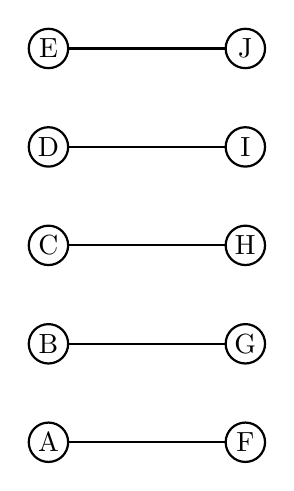
\begin{tikzpicture}[scale=2.5]
\coordinate (A) at (0,0);
\coordinate (B) at (0,0.5);
\coordinate (C) at (0,1);
\coordinate (D) at (0,1.5);
\coordinate (E) at (0,2);
\coordinate (F) at (1,0);
\coordinate (G) at (1,0.5);
\coordinate (H) at (1,1);
\coordinate (I) at (1,1.5);
\coordinate (J) at (1,2);
\draw[thick] (A) -- (F);
\draw[thick] (B) -- (G);
\draw[thick] (C) -- (H);
\draw[thick] (D) -- (I);
\draw[thick] (E) -- (J);
\draw[thick, fill=white] (A) circle (0.1) node {A};
\draw[thick, fill=white] (B) circle (0.1) node {B};
\draw[thick, fill=white] (C) circle (0.1) node {C};
\draw[thick, fill=white] (D) circle (0.1) node {D};
\draw[thick, fill=white] (E) circle (0.1) node {E};
\draw[thick, fill=white] (F) circle (0.1) node {F};
\draw[thick, fill=white] (G) circle (0.1) node {G};
\draw[thick, fill=white] (H) circle (0.1) node {H};
\draw[thick, fill=white] (I) circle (0.1) node {I};
\draw[thick, fill=white] (J) circle (0.1) node {J};
\end{tikzpicture}
\end{center}
}
\end{column}
\end{columns}
\end{frame}

\begin{frame}
\frametitle{1 fokú csúcsok}

\begin{columns}
\begin{column}{0.5\textwidth}
\begin{footnotesize}
\begin{itemize}
\item
\only<-2>{Csúcsok száma: $n\leq{}2k^2$}
\only<3->{Csúcsok száma: $n$ $\textcolor{red}{\leq{}k^2}$}
(pl. $1000$)
\item Élek száma: $e\leq{}k^2$
\item Kizárható vendégek száma: $k$ (pl. $10$)
\item \only<1>{Csúcsok fokszáma: $1\leq{}d(v)\leq{}k$}\only<2->{Csúcsok fokszáma: $\textcolor{red}{2\leq{}}d(v)\leq{}k$}
\end{itemize}
\emptyline
Mit tehetünk a következő csúcsokkal?
\begin{itemize}
\item A: $1$ fokszámú csúcs \uncover<2->{\textcolor{red}{$\rightarrow$ Beengedjük}}
\item B: A szomszédja \uncover<2->{\textcolor{red}{$\rightarrow$ Kitiltjuk, k-t csökkentjük}}
\end{itemize}

\begin{itemize}
\uncover<4->{\item ${{k^2}\choose{k}}$, pl. ${{100}\choose{10}} \approx 1.73\cdot10^{13}$.\\
Már a laptopunk is le tudja futtatni!}
\end{itemize}
\end{footnotesize}
\end{column}

\begin{column}{0.5\textwidth}
\begin{center}
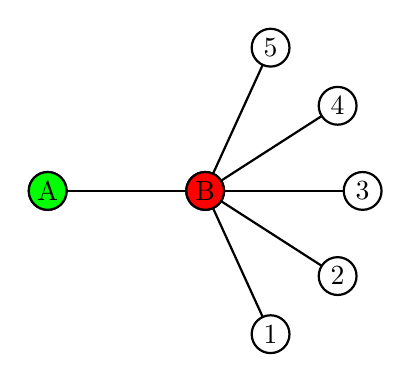
\begin{tikzpicture}[scale=2]
\coordinate (N1) at (1.41542,0.09037);
\coordinate (N2) at (1.84125,0.45936);
\coordinate (N3)  at (2.00000,1.00000);
\coordinate (N4)  at (1.84125,1.54064);
\coordinate (N5)  at (1.41542,1.90963);
\coordinate (A)   at (0.00000,1.00000);
\coordinate (B)   at (1.00000,1.00000);
\draw[thick] (B) -- (N1);
\draw[thick] (B) -- (N2);
\draw[thick] (B) -- (N3);
\draw[thick] (B) -- (N4);
\draw[thick] (B) -- (N5);
\draw[thick] (A) -- (B);
\draw[thick, fill=white] (N1)  circle (0.12) node{1};
\draw[thick, fill=white] (N2)  circle (0.12) node{2};
\draw[thick, fill=white] (N3)  circle (0.12) node{3};
\draw[thick, fill=white] (N4)  circle (0.12) node{4};
\draw[thick, fill=white] (N5)  circle (0.12) node{5};
\uncover<1>{\draw[thick, fill=white] (A)   circle (0.12) node {A};}
\uncover<2->{\draw[thick, fill=green] (A)   circle (0.12) node {A};}
\uncover<1>{\draw[thick, fill=white] (B)   circle (0.12) node {B};}
\uncover<2->{\draw[thick, fill=red]   (B)   circle (0.12) node {B};}
\end{tikzpicture}
\end{center}
\end{column}
\end{columns}

\end{frame}


\begin{frame}
\frametitle{Folytatás}

Bounded Search Trees

\end{frame}


\section{Definíciók}
\begin{frame}
\frametitle{Etc}
\end{frame}

\section{Feedback Arc Set problem}
\begin{frame}
\frametitle{Tournament gráf}

Irányított gráf, minden csúcspárra pontosan 1 irányban van él.

\begin{center}
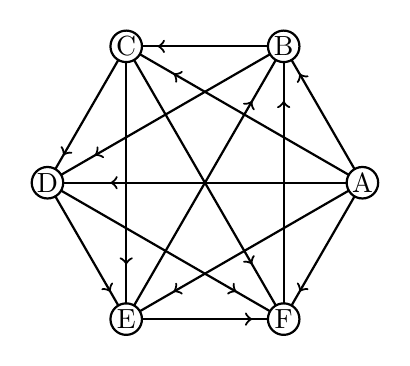
\begin{tikzpicture}[scale=2]
\coordinate (A) at (2.00000,1.00000);
\coordinate (B) at (1.50000,1.86603);
\coordinate (C) at (0.50000,1.86603);
\coordinate (D) at (0.00000,1.00000);
\coordinate (E) at (0.50000,0.13397);
\coordinate (F) at (1.50000,0.13397);

\begin{scope}[thick,decoration={
    markings,
    mark=at position 0.8 with {\arrow{>}}}
    ] 
    \draw[thick, postaction={decorate}] (A) -- (B);
    \draw[thick, postaction={decorate}] (A) -- (C);
    \draw[thick, postaction={decorate}] (A) -- (D);
    \draw[thick, postaction={decorate}] (A) -- (E);
    \draw[thick, postaction={decorate}] (A) -- (F);
    \draw[thick, postaction={decorate}] (B) -- (C);
    \draw[thick, postaction={decorate}] (B) -- (D);
    \draw[thick, postaction={decorate}] (E) -- (B);
    \draw[thick, postaction={decorate}] (F) -- (B);
    \draw[thick, postaction={decorate}] (C) -- (D);
    \draw[thick, postaction={decorate}] (C) -- (E);
    \draw[thick, postaction={decorate}] (C) -- (F);
    \draw[thick, postaction={decorate}] (D) -- (E);
    \draw[thick, postaction={decorate}] (D) -- (F);
    \draw[thick, postaction={decorate}] (E) -- (F);
\end{scope}
\draw[thick, fill=white] (A) circle (0.1) node {A};
\draw[thick, fill=white] (B) circle (0.1) node {B};
\draw[thick, fill=white] (C) circle (0.1) node {C};
\draw[thick, fill=white] (D) circle (0.1) node {D};
\draw[thick, fill=white] (E) circle (0.1) node {E};
\draw[thick, fill=white] (F) circle (0.1) node {F};
\end{tikzpicture}
\end{center}
\end{frame}

\begin{frame}
\frametitle{Feedback arc set}

\begin{itemize}
\item Olyan élhalmaz, amit ha megfordítok nem lesz kör a gráfban.
\item Tehát a gráf minden körének legalább az egyik éle benne van.
\item Feladat: legfeljebb k elemű feedback arc set találása.
\end{itemize}

\begin{center}
\begin{tikzpicture}[scale=2]
\coordinate (A) at (2.00000,1.00000);
\coordinate (B) at (1.50000,1.86603);
\coordinate (C) at (0.50000,1.86603);
\coordinate (D) at (0.00000,1.00000);
\coordinate (E) at (0.50000,0.13397);
\coordinate (F) at (1.50000,0.13397);

\begin{scope}[thick,decoration={
    markings,
    mark=at position 0.8 with {\arrow{>}}}
    ] 
    \draw[thick, postaction={decorate}] (A) -- (B);
    \draw[thick, postaction={decorate}] (A) -- (C);
    \draw[thick, postaction={decorate}] (A) -- (D);
    \draw[thick, postaction={decorate}] (A) -- (E);
    \draw[thick, postaction={decorate}] (A) -- (F);
    \draw[thick, postaction={decorate}] (B) -- (C);
    \draw[thick, postaction={decorate}] (B) -- (D);
\only<1>{\draw[thick, red, postaction={decorate}] (E) -- (B);}
\only<2>{\draw[thick, blue, postaction={decorate}] (B) -- (E);}
\only<1>{\draw[thick, red, postaction={decorate}] (F) -- (B);}
\only<2>{\draw[thick, blue, postaction={decorate}] (B) -- (F);}
    \draw[thick, postaction={decorate}] (C) -- (D);
    \draw[thick, postaction={decorate}] (C) -- (E);
    \draw[thick, postaction={decorate}] (C) -- (F);
    \draw[thick, postaction={decorate}] (D) -- (E);
    \draw[thick, postaction={decorate}] (D) -- (F);
    \draw[thick, postaction={decorate}] (E) -- (F);
\end{scope}
\draw[thick, fill=white] (A) circle (0.1) node {A};
\draw[thick, fill=white] (B) circle (0.1) node {B};
\draw[thick, fill=white] (C) circle (0.1) node {C};
\draw[thick, fill=white] (D) circle (0.1) node {D};
\draw[thick, fill=white] (E) circle (0.1) node {E};
\draw[thick, fill=white] (F) circle (0.1) node {F};
\end{tikzpicture}
\end{center}
\end{frame}

\begin{frame}
\frametitle{Kernelizáció: 1. szabály}

Ha egy él k+1 háromszögben is benne van, akkor fordítsuk meg.

\begin{center}
\begin{tikzpicture}[scale=2]
\coordinate (A) at (2.00000,1.00000);
\coordinate (B) at (1.50000,1.86603);
\coordinate (C) at (0.50000,1.86603);
\coordinate (D) at (0.00000,1.00000);
\coordinate (E) at (0.50000,0.13397);
\coordinate (F) at (1.50000,0.13397);

\begin{scope}[thick,decoration={
    markings,
    mark=at position 0.8 with {\arrow{>}}}
    ] 
    \draw[thick, postaction={decorate}] (A) -- (E);
    \draw[thick, postaction={decorate}] (B) -- (E);
    \draw[thick, postaction={decorate}] (C) -- (E);
    \draw[thick, postaction={decorate}] (D) -- (E);
    \draw[thick, postaction={decorate}] (F) -- (A);
    \draw[thick, postaction={decorate}] (F) -- (B);
    \draw[thick, postaction={decorate}] (F) -- (C);
    \draw[thick, postaction={decorate}] (F) -- (D);
    \only<1>{\draw[thick, red,  postaction={decorate}] (E) -- (F);}
    \only<2>{\draw[thick, blue, postaction={decorate}] (F) -- (E);}
\end{scope}
\draw[thick, fill=white] (A) circle (0.1) node {A};
\draw[thick, fill=white] (B) circle (0.1) node {B};
\draw[thick, fill=white] (C) circle (0.1) node {C};
\draw[thick, fill=white] (D) circle (0.1) node {D};
\draw[thick, fill=white] (E) circle (0.1) node {E};
\draw[thick, fill=white] (F) circle (0.1) node {F};
\end{tikzpicture}
\end{center}
\end{frame}

\begin{frame}
\frametitle{Kernelizáció: 2. szabály}

Ha egy csúcs nincs benne egyetlen háromszögben sem, akkor töröljük.
\begin{itemize}
\item \uncover<2->{A v nincs benne egyetlen körben sem.}
\item \uncover<3->{Az Y $\rightarrow$ v, illetve v $\rightarrow$ X élekre nincs szükség a feedback arc setben.}
\item \uncover<4->{Az Y $\rightarrow$ X élek nem fognak megfordulni.}
\end{itemize}

\begin{center}
\begin{tikzpicture}[scale=1.5]
\coordinate (V) at (0,1);
\coordinate (X) at (2,0);
\coordinate (Xl) at (1.6,0);
\coordinate (Xlc) at (1.8,0);
\coordinate (Xr) at (2.4,0);
\coordinate (Xrc) at (2.2,0);
\coordinate (Y) at (2,2);
\coordinate (Yl) at (1.6,2);
\coordinate (Ylc) at (1.8,2);
\coordinate (Yr) at (2.4,2);
\coordinate (Yrc) at (2.2,2);

\begin{scope}[thick,decoration={
    markings,
    mark=at position 0.5 with {\arrow{>}}}
    ] 
    \only<-4>{\draw[thick, postaction={decorate}] (V) -- (Xl);}
    \only<-4>{\draw[thick, postaction={decorate}] (V) -- (X);}
    \only<-4>{\draw[thick, postaction={decorate}] (V) -- (Xr);}
    \only<-4>{\draw[thick, postaction={decorate}] (Yl) -- (V);}
    \only<-4>{\draw[thick, postaction={decorate}] (Y) -- (V);}
    \only<-4>{\draw[thick, postaction={decorate}] (Yr) -- (V);}
    \draw[thick, postaction={decorate}] (Ylc) -- (Xlc);
    \draw[thick, postaction={decorate}] (Y) -- (X);
    \draw[thick, postaction={decorate}] (Yrc) -- (Xrc);
\end{scope}
\only<-4>{\draw[thick, fill=white] (V) circle (0.1) node {v};}
\draw[thick, fill=white] (X) circle (0.5) node {X};
\only<-5>{\draw[thick, fill=white] (Y) circle (0.5) node {Y};}
\end{tikzpicture}
\end{center}

\end{frame}

\begin{frame}
\frametitle{Kernel mérete}
\begin{itemize}
\item Alkalmazzuk ezeket a szabályokat amíg lehet.
\pause
\item Amikor már nem lehet:
\begin{itemize}
\item 1. szabályt nem lehet, mert: minden él legfeljebb k háromszög része.
\item 2. szabály nem lehet, mert: minden csúcs része valamely háromszögnek.
\pause
\end{itemize}
\begin{footnotesize}
\item Tfh. van k méretű feedback arc set: F.\pause
\item Ennek egy élére: 2 végpont + k db csúccsal lehet háromszögben (1. szabály nem alkalmazható)\pause
\item Minden csúcs benne van egy háromszögben (2. szabály nem alkalmazható)\pause
\item Minden háromszögben van él F-ből. \pause
\item Leszámláltunk k db F-beli élre darabonként k+2 csúcsot, kihagyás nélkül.\pause
\item A gráfban legfeljebb $k(k+2)$ csúcs van, ha megoldható.
\end{footnotesize}
\end{itemize}
\end{frame}


\section{Felhasznált irodalom}
\begin{frame}
\begin{center}
\includegraphics[height=0.9\textheight]{book.png}
\end{center}
\end{frame}

\end{document}
